\documentclass[usenames,dvipsnames]{beamer}
\usetheme{its}
\usepackage[utf8]{inputenc}
\usepackage[T1]{fontenc}
\usepackage[english]{babel}

\usepackage{amsmath}
\usepackage{amsfonts}
\usepackage{amssymb}
\usepackage{amsthm}
\usepackage{csquotes}
\usepackage{tikz}

\usetikzlibrary{arrows,automata}

%\setbeamercolor{sidebar}{fg=white,bg=white}
\setbeamertemplate{footline}[frame number]
\beamertemplatenavigationsymbolsempty

\newcommand{\cstit}{\operatorname{cstit}}

\title{Challenges with Obligations in Multiagent Deontic Logic}
\subtitle{Challenges 2, 3 and 4}
\author{Raik Hipler and Mark Scheibner}
\date{11.03.2021}



\begin{document}
    \begingroup
    \makeatletter
    \setlength{\hoffset}{.5\beamer@sidebarwidth}
    \makeatother
    \frame[plain]{\titlepage}
    \endgroup
	
	\begin{frame}[plain]
		\frametitle{Outline}
		\tableofcontents
	\end{frame}
    
    \section{Introduction}
	\begin{frame}{Introduction}
		\framesubtitle{Ought-to-be and Ought-to-do}
		\begin{itemize}
		    \item SDL and DSDL give us frameworks for handling how things \emph{ought to be}
		    \item Since we are interested in the actions of agents, we need to describe what agents \emph{ought to do}
		    \item Simply redefining \emph{ought to do} as \emph{ought to be done} leads to various problems
		\end{itemize}
	\end{frame}
	
	\begin{frame}{STIT logic}
	    \begin{itemize}
		    \item STIT trees model possible decisions of (multiple) agents
		    \item Inner node are sets of actions the agent has to decide between
		    \item Each action may non-deterministically lead to different outcomes
		    \item Leafs are histories with associated utility values
		\end{itemize}
		\pause
	    \begin{figure}[ht]
            \centering
            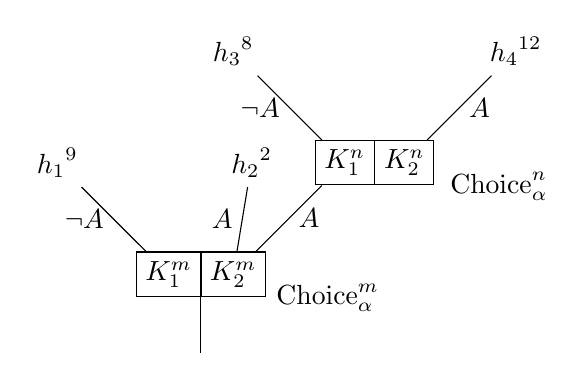
\begin{tikzpicture}[node distance=2cm]
                \node (start) {};
                \node[draw,rectangle] (choice11) [above of=start, yshift=-1cm] {$K_1^m$};
                \node[draw,rectangle] (choice12) [right of=choice11,xshift=-1.18cm] {$K_2^m$};
                \node (choicem) [right of=choice12,yshift=-0.3cm,xshift=-0.8cm] {$\text{Choice}_\alpha^m$};
                \node (h1) [above left of=choice11] {${h_1}^9$};
                \node (h2) [above right of=choice12,xshift=-1.18cm] {${h_2}^2$};
                \node[draw,rectangle] (choice21) [above right of=choice12] {$K_1^n$};
                \node[draw,rectangle] (choice22) [right of=choice21,xshift=-1.24cm] {$K_2^n$};
                \node (choicen) [right of=choice22,yshift=-0.3cm,xshift=-0.8cm] {$\text{Choice}_\alpha^n$};
                \node (h3) [above left of=choice21] {${h_3}^8$};
                \node (h4) [above right of=choice22] {${h_4}^{12}$};
            
                \draw
                ([xshift=.4cm]start.center) edge ([xshift=.4cm]choice11.center)
                (choice12) edge node[left] {$A$} (h2)
                (choice12) edge node[right] {$A$} (choice21)
                (choice21) edge node[left] {$\lnot A$} (h3)
                (choice22) edge node[right] {$A$} (h4)
                (choice11) edge node[left] {$\lnot A$} (h1);
            \end{tikzpicture}
        \end{figure}
	\end{frame}
	
	\begin{frame}{STIT logic}
	    \framesubtitle{Semantics}
	    \begin{figure}[ht]
            \centering
            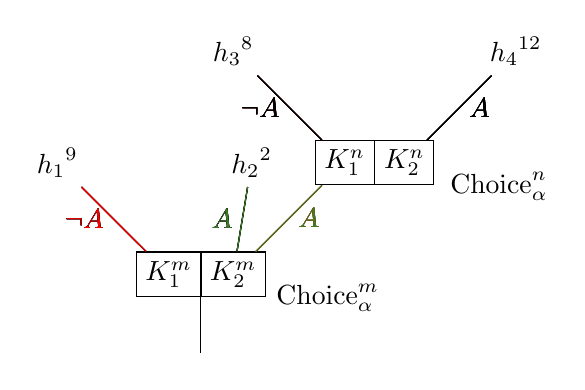
\begin{tikzpicture}[node distance=2cm]
                \node (start) {};
                \node[draw,rectangle] (choice11) [above of=start, yshift=-1cm] {$K_1^m$};
                \node[draw,rectangle] (choice12) [right of=choice11,xshift=-1.18cm] {$K_2^m$};
                \node (choicem) [right of=choice12,yshift=-0.3cm,xshift=-0.8cm] {$\text{Choice}_\alpha^m$};
                \node (h1) [above left of=choice11] {${h_1}^9$};
                \node (h2) [above right of=choice12,xshift=-1.18cm] {${h_2}^2$};
                \node[draw,rectangle] (choice21) [above right of=choice12] {$K_1^n$};
                \node[draw,rectangle] (choice22) [right of=choice21,xshift=-1.24cm] {$K_2^n$};
                \node (choicen) [right of=choice22,yshift=-0.3cm,xshift=-0.8cm] {$\text{Choice}_\alpha^n$};
                \node (h3) [above left of=choice21] {${h_3}^8$};
                \node (h4) [above right of=choice22] {${h_4}^{12}$};
            
                \draw<1-2,4,7>
                ([xshift=.4cm]start.center) edge ([xshift=.4cm]choice11.center)
                (choice12) edge node[left] {$A$} (h2)
                (choice12) edge node[right] {$A$} (choice21)
                (choice21) edge node[left] {$\lnot A$} (h3)
                (choice22) edge node[right] {$A$} (h4)
                (choice11) edge node[left] {$\lnot A$} (h1);
                \draw<3>
                ([xshift=.4cm]start.center) edge ([xshift=.4cm]choice11.center)
                (choice12) edge node[left] {$A$} (h2)
                (choice12) edge[color=OliveGreen] node[right] {$A$} (choice21)
                (choice21) edge[color=red] node[left] {$\lnot A$} (h3)
                (choice22) edge node[right] {$A$} (h4)
                (choice11) edge node[left] {$\lnot A$} (h1);
                \draw<5>
                ([xshift=.4cm]start.center) edge ([xshift=.4cm]choice11.center)
                (choice12) edge node[left] {$A$} (h2)
                (choice12) edge[color=OliveGreen] node[right] {$A$} (choice21)
                (choice21) edge node[left] {$\lnot A$} (h3)
                (choice22) edge node[right] {$A$} (h4)
                (choice11) edge node[left] {$\lnot A$} (h1);
                \draw<6>
                ([xshift=.4cm]start.center) edge ([xshift=.4cm]choice11.center)
                (choice12) edge node[left] {$A$} (h2)
                (choice12) edge[color=red] node[right] {$A$} (choice21)
                (choice21) edge node[left] {$\lnot A$} (h3)
                (choice22) edge node[right] {$A$} (h4)
                (choice11) edge node[left] {$\lnot A$} (h1);
                \draw<8>
                ([xshift=.4cm]start.center) edge ([xshift=.4cm]choice11.center)
                (choice12) edge[color=OliveGreen] node[left] {$A$} (h2)
                (choice12) edge[color=OliveGreen] node[right] {$A$} (choice21)
                (choice21) edge node[left] {$\lnot A$} (h3)
                (choice22) edge node[right] {$A$} (h4)
                (choice11) edge[color=red] node[left] {$\lnot A$} (h1);
            \end{tikzpicture}
            
        \end{figure}
        \only<1>{\begin{itemize}
            \item Consider moment-history pairs
            \item Does $m,h\models \varphi$ hold?
        \end{itemize}}
        
        \only<2-3>{Atomic propositions}
        \only<2>{\begin{itemize}
            \item $m,h_3\models A$?
            \item $n,h_3\models A$?
        \end{itemize}}
        \only<3>{\begin{itemize}
            \item \color{OliveGreen} $m,h_3\models A$
            \item \color{red} $n,h_3\not\models A$
        \end{itemize}}
        
        \only<4-6>{Obligations}
        \only<4>{\begin{itemize}
            \item $m,h_2\models \bigcirc A$?
            \item $m,h_2\models \bigcirc\neg A$?
        \end{itemize}}
        \only<5>{\begin{itemize}
            \item {\color{OliveGreen} $m,h_2\models \bigcirc A$}
            \item $m,h_2\models \bigcirc\neg A$
        \end{itemize}}
        \only<6>{\begin{itemize}
            \item $m,h_2\models \bigcirc A$
            \item \color{red} $m,h_2\not\models \bigcirc\neg A$
        \end{itemize}}
        
        \only<7-8>{See-To-It-That}
        \only<7>{\begin{itemize}
            \item $m,h_3\models [\alpha\cstit\colon A]$?
            \item $m,h_1\models [\alpha\cstit\colon A]$?
        \end{itemize}}
        \only<8>{\begin{itemize}
            \item \color{OliveGreen} $m,h_3\models [\alpha\cstit\colon A]$
            \item \color{red} $m,h_1\not\models [\alpha\cstit\colon A]$
        \end{itemize}}
	\end{frame}

    \section{Non-Deterministic Actions}
    \begin{frame}{Challenge 2: Non-Deterministic Actions}
        How can we deal with different possible outcomes caused by non-determinism?
	\end{frame}
	
	\begin{frame}{Challenge 2: Non-Deterministic Actions}
		\framesubtitle{The gambling problem}
		\begin{itemize}
		    \item The agent is presented with two options
		    \item If he gambles, he can either double or lose his bet
		    \item If he does not gamble, he preserves his money
		\end{itemize}
		\pause
		\begin{figure}[ht]
            \centering
             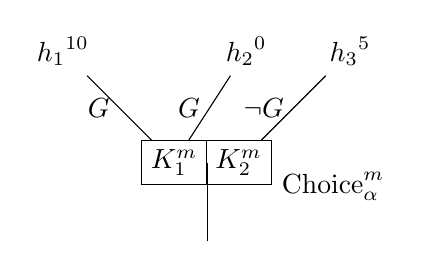
\begin{tikzpicture}[node distance=2cm]
                \node (start) {};
                \node[draw,rectangle] (choice11) [above of=start, yshift=-1cm] {$K_1^m$};
                \node[draw,rectangle] (choice12) [right of=choice11,xshift=-1.18cm] {$K_2^m$};
                \node (choicem) [right of=choice12,yshift=-0.3cm,xshift=-0.8cm] {$\text{Choice}_\alpha^m$};
                \node (h1) [above left of=choice11] {${h_1}^{10}$};
                \node (h2) [above right of=choice11, xshift=-.5cm] {${h_2}^0$};
                \node (h3) [above right of=choice12] {${h_3}^5$};
                
                \draw
                ([xshift=.42cm]start.center) edge ([xshift=.42cm]choice11.center)
                (choice11) edge node[left] {$G$} (h1)
                (choice11) edge node[left] {$G$} (h2)
                (choice12) edge node[left] {$\neg G$} (h3);
            \end{tikzpicture}
        \end{figure}
        How can we formulate that the agent should arrive at $h_1$?
	\end{frame}
	
	\begin{frame}{Challenge 2: Non-Deterministic Actions}
		\framesubtitle{Optimality of non-deterministic actions}
		\begin{itemize}
		    \item The optimal path ends in $h_1$
		    \item The agent should \enquote{ought to see to it that G}
		    \item Intuitive formulation $\bigcirc[\alpha \cstit \colon G]$ problematic since $K_1^m$ is not necessarily better than $K_2^m$\pause
		    \item We cannot infer optimal actions from optimal histories
		    \item An action may lead non-deterministically to worse histories
		\end{itemize}
	\end{frame}
	
	\begin{frame}{Challenge 2: Non-Deterministic Actions}
		%\framesubtitle{Optimality of non-deterministic actions}
		More appropriate approach:
		\begin{itemize}
		    \item Compare all possible histories
		    \item $K_1$ is more optimal than $K_2$ if it has one history that is better than every history of $K_2$ and no worse history
		\end{itemize}
		\pause
		New operator: $\odot [\alpha \cstit \colon G]$
		\begin{itemize}
		    \item Fulfilled if no action not leading to $G$ is the optimal action
		    \item Back to the gambling problem:\\ Neither $\odot [\alpha \cstit \colon G]$ nor $\odot [\alpha \cstit \colon \neg G]$ hold for $m$
		\end{itemize}
		\begin{figure}[ht]
            \centering
            \scalebox{.8}{
                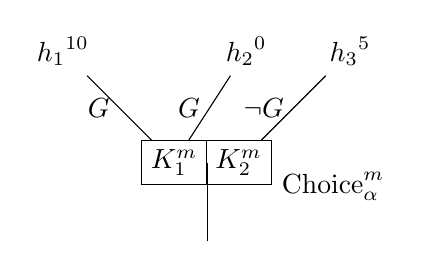
\begin{tikzpicture}[node distance=2cm]
                \node (start) {};
                \node[draw,rectangle] (choice11) [above of=start, yshift=-1cm] {$K_1^m$};
                \node[draw,rectangle] (choice12) [right of=choice11,xshift=-1.18cm] {$K_2^m$};
                \node (choicem) [right of=choice12,yshift=-0.3cm,xshift=-0.8cm] {$\text{Choice}_\alpha^m$};
                \node (h1) [above left of=choice11] {${h_1}^{10}$};
                \node (h2) [above right of=choice11, xshift=-.5cm] {${h_2}^0$};
                \node (h3) [above right of=choice12] {${h_3}^5$};
                
                \draw
                ([xshift=.42cm]start.center) edge ([xshift=.42cm]choice11.center)
                (choice11) edge node[left] {$G$} (h1)
                (choice11) edge node[left] {$G$} (h2)
                (choice12) edge node[left] {$\neg G$} (h3);
            \end{tikzpicture}}
        \end{figure}
	\end{frame}
    
    \section{Moral Luck}
    \begin{frame}
		\frametitle{Challenge 3: Moral Luck}
	
		How do we deal with luck?
	
	\end{frame}

	\begin{frame}
		\frametitle{Challenge 3: Moral Luck}

		\begin{itemize}
			\item Sometimes the consequences of our actions are outside of our control
			\item This may for example happen if the outcome is also dependent on someone else's actions\pause
			\item How do we evaluate the formula $\odot [\alpha \cstit \colon A]$ if the outcome also depends on another agents decision?
		\end{itemize}
	
	\end{frame}

	\begin{frame}
		\frametitle{Challenge 3: Moral Luck}
		\framesubtitle{The driving example}

		\begin{itemize}
			\item Two cars are driving towards each other on a small road
			\item The drivers ($\alpha$ and $\beta$) both have to decide whether to swerve to the side ($S$) or drive straight ($\lnot S$)\pause
			\item If both decide on the same action, they will crash
			\item How do we deal with $\odot [\alpha \cstit \colon S]$?
		\end{itemize}

		\begin{figure}[ht]
            \centering
             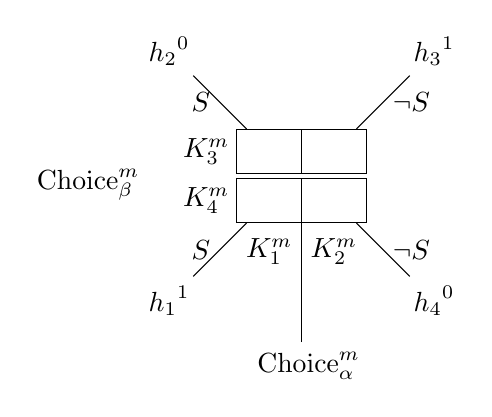
\begin{tikzpicture}[node distance=1.8cm]
                \node (start) {};
                \node[draw,rectangle,text opacity=0] (choice11) [above of=start] {$K_1^m$};
                \node (K1) [below of=choice11, yshift=1.15cm] {$K_1^m$};
                \node[draw,rectangle, text opacity=0] (choice12) [right of=choice11,xshift=-0.98cm] {$K_2^m$};
                \node (K2) [below of=choice12, yshift=1.15cm] {$K_2^m$};
                \node[draw,rectangle, text opacity=0] (choice13) [above of=choice11,yshift=-1.18cm] {$K_3^m$};
                \node (K3) [left of=choice13, xshift=1cm] {$K_3^m$};
                \node[draw,rectangle, text opacity=0] (choice14) [right of=choice13,xshift=-0.98cm] {$K_4^m$};
                \node (K4) [left of=choice11, xshift=1cm] {$K_4^m$};
                
                \node (choicem) [below of=start, yshift=1.5cm, xshift=.5cm] {$\text{Choice}_\alpha^m$};
                \node (choicen) [left of=choice11, yshift=.2cm, xshift=-.5cm] {$\text{Choice}_\beta^m$};
                \node (h1) [below left of=choice11] {${h_1}^1$};
                \node (h2) [above left of=choice13] {${h_2}^0$};
                \node (h3) [above right of=choice14] {${h_3}^1$};
                \node (h4) [below right of=choice12] {${h_4}^0$};
                
                \draw
                ([xshift=.41cm]start.center) edge ([xshift=.41cm]choice11.center)
                (choice11) edge node[left] {$S$} (h1)
                (choice12) edge node[right] {$\neg S$} (h4)
                (choice13) edge node[left] {$S$} (h2)
                (choice14) edge node[right] {$\neg S$} (h3);
            \end{tikzpicture}
        \end{figure}
 	\end{frame}
    
    \begin{frame}
        \frametitle{Challenge 3: Moral Luck}

        There are two views:\pause
        \begin{itemize}
            \item Dominance act utilitarianism: \pause
            \begin{itemize}
                \item $\odot [\alpha \cstit \colon S]$ if all optimal outcomes guarantee $S$
                \item In the example this is not the case, since $\lnot S$ can also lead to an optimal outcome
                \item The same goes for $\odot [\alpha \cstit \colon \lnot S]$
            \end{itemize} \pause
            \item Orthodox perspective\pause
            \begin{itemize}
                \item We don't evaluate the formula at the time of $m$
                \item We decide whether $\odot [\alpha \cstit \colon S]$ should be true based on the outcome
                \item Intuitively, we ask whether $\alpha$ \emph{should have} swerved
            \end{itemize}
        \end{itemize}

    \end{frame}
    
    \section{Procrastination}
	\begin{frame}
		\frametitle{Challenge 4: Procrastination}
	
		How do we deal with actions that will never be taken?
	
	\end{frame}

	\begin{frame}
		\frametitle{Challenge 4: Procrastination}
	
		\begin{itemize}
			\item Agents can put off on following through with obligations
			\item Since they can do so over and over, tasks need deadlines
			\begin{itemize}
				\item See also: Thread Starvation
			\end{itemize}
			\item But what if agents still procrastinate?
		\end{itemize}
	
	\end{frame}

	\begin{frame}
		\frametitle{Challenge 4: Procrastination}
		\framesubtitle{The story of Professor Procrastinate}

		\begin{itemize}
			\item Professor Procrastinate is requested to write a review
			\item He is the best person available for writing the review
			\item He is known to procrastinate and will not actually write the review
			\item Should Professor Procrastinate accept the request?
		\end{itemize}\pause

		We now run into a paradox:\pause
		\begin{itemize}
			\item He ought to accept since him writing the review is the best scenario\pause
			\item He ought to decline since he will not actually write the review, which leads to the worst outcome
		\end{itemize}
	\end{frame}

	\begin{frame}
		\frametitle{Challenge 4: Procrastination}

		The solution: Just prune the branch!
		\begin{figure}[ht]
			\centering
			\only<1>{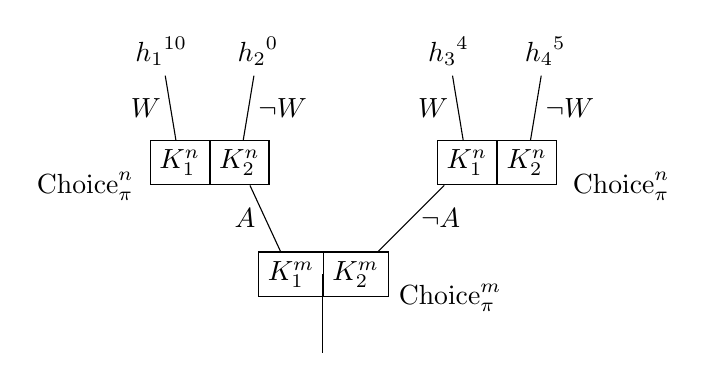
\begin{tikzpicture}[node distance=2cm]
				\node (start) {};
				\node[draw,rectangle] (choice11) [above of=start, yshift=-1cm] {$K_1^m$};
				\node[draw,rectangle] (choice12) [right of=choice11,xshift=-1.18cm] {$K_2^m$};
				\node (choicem) [right of=choice12,yshift=-0.3cm,xshift=-0.8cm] {$\text{Choice}_\pi^m$};

				\node[draw,rectangle] (choice21A) [above left of=choice11] {$K_1^n$};
				\node[draw,rectangle] (choice22A) [right of=choice21A,xshift=-1.24cm] {$K_2^n$};
				\node (choicenA) [right of=choice21A,yshift=-0.3cm,xshift=-3.2cm] {$\text{Choice}_\pi^n$};
				\node (h1) [above left of=choice21A,xshift=1.18cm] {${h_1}^{10}$};
				\node (h2) [above right of=choice22A,xshift=-1.18cm] {${h_2}^0$};

				\node[draw,rectangle] (choice21B) [above right of=choice12] {$K_1^n$};
				\node[draw,rectangle] (choice22B) [right of=choice21B,xshift=-1.24cm] {$K_2^n$};
				\node (choicenB) [right of=choice22B,yshift=-0.3cm,xshift=-0.8cm] {$\text{Choice}_\pi^n$};
				\node (h3) [above left of=choice21B,xshift=1.18cm] {${h_3}^4$};
				\node (h4) [above right of=choice22B,xshift=-1.18cm] {${h_4}^{5}$};
				
				\draw
				([xshift=.4cm]start.center) edge ([xshift=.4cm]choice11.center)
				(choice11) edge node[left] {$A$} (choice22A)
				(choice12) edge node[right] {$\lnot A$} (choice21B)
				(choice21A) edge node[left] {$W$} (h1)
				(choice22A) edge node[right] {$\lnot W$} (h2)
				(choice21B) edge node[left] {$W$} (h3)
				(choice22B) edge node[right] {$\lnot W$} (h4);
			\end{tikzpicture}}
			
			\only<2>{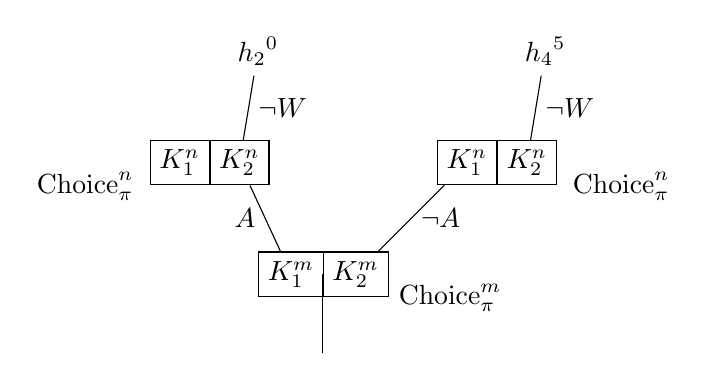
\begin{tikzpicture}[node distance=2cm]
				\node (start) {};
				\node[draw,rectangle] (choice11) [above of=start, yshift=-1cm] {$K_1^m$};
				\node[draw,rectangle] (choice12) [right of=choice11,xshift=-1.18cm] {$K_2^m$};
				\node (choicem) [right of=choice12,yshift=-0.3cm,xshift=-0.8cm] {$\text{Choice}_\pi^m$};

				\node[draw,rectangle] (choice21A) [above left of=choice11] {$K_1^n$};
				\node[draw,rectangle] (choice22A) [right of=choice21A,xshift=-1.24cm] {$K_2^n$};
				\node (choicenA) [right of=choice21A,yshift=-0.3cm,xshift=-3.2cm] {$\text{Choice}_\pi^n$};
				\node (h2) [above right of=choice22A,xshift=-1.18cm] {${h_2}^0$};

				\node[draw,rectangle] (choice21B) [above right of=choice12] {$K_1^n$};
				\node[draw,rectangle] (choice22B) [right of=choice21B,xshift=-1.24cm] {$K_2^n$};
				\node (choicenB) [right of=choice22B,yshift=-0.3cm,xshift=-0.8cm] {$\text{Choice}_\pi^n$};
				\node (h4) [above right of=choice22B,xshift=-1.18cm] {${h_4}^{5}$};
				
				\draw
				([xshift=.4cm]start.center) edge ([xshift=.4cm]choice11.center)
				(choice11) edge node[left] {$A$} (choice22A)
				(choice12) edge node[right] {$\lnot A$} (choice21B)
				(choice22A) edge node[right] {$\lnot W$} (h2)
				(choice22B) edge node[right] {$\lnot W$} (h4);
			\end{tikzpicture}}
			
			\only<3>{\begin{tikzpicture}[node distance=2cm]
				\node (start) {};
				\node[draw,rectangle] (choice11) [above of=start, yshift=-1cm] {$K_1^m$};
				\node[draw,rectangle] (choice12) [right of=choice11,xshift=-1.18cm] {$K_2^m$};
				\node (choicem) [right of=choice12,yshift=-0.3cm,xshift=-0.8cm] {$\text{Choice}_\pi^m$};

				\node (h2) [above right of=choice22A,xshift=-1.18cm] {${h_2}^0$};
				\node (h4) [above right of=choice22B,xshift=-1.18cm] {${h_4}^{5}$};

				\draw
				([xshift=.4cm]start.center) edge ([xshift=.4cm]choice11.center)
				(choice11) edge node[left] {$A$} (h2)
				(choice12) edge node[right] {$\lnot A$} (h4);
			\end{tikzpicture}}
		\end{figure}
	\end{frame}

    \section{Summary}
    \begin{frame}
        \frametitle{Summary}
    
        \begin{itemize}
            \item For the gambling problem we can circumvent the problem by modifying the semantics
            \begin{itemize}
                \item Instead of considering only the best outcome we consider every possible outcome
            \end{itemize}
            \item We we're unable to solve the driving example
            \begin{itemize}
                \item Instead two perspectives on how the semantics should work were given
                \item Which one is to be used is a design decision
            \end{itemize}
            \item The problem of procrastination can be solved by using additional knowledge to cut branches from the STIT-tree
        \end{itemize}
    
    \end{frame}
    

\end{document}